\documentclass{article}
\usepackage[utf8]{inputenc}
\usepackage{amsmath}
\usepackage{graphicx}
    \DeclareGraphicsExtensions{.png, .jpeg}
\usepackage{caption}
\usepackage[top=1in, bottom=1in, left=1in, right=1in]{geometry}
\setlength{\parindent}{0pt}

\title{Smok3 Tagg3r: A Lightweight Graphical Interface Application for Creating or Verifying Image Annotations Manually}
\author{Terence Henriod}
\date{\today}

\begin{document}
%
\clearpage            % All of
\maketitle            % this,
\thispagestyle{empty} % removes the page number from the title page
%
\begin{abstract}
In this document we discuss the usage of the lightweight GUI application created to aid in marking images for training computer vision applications.
\end{abstract}

\newpage
%%%%%%%%%%%%%%%%%%%%%%%%%%%%%%%%%%%%%%%%%%%%%%%%%%%%%%%%%%%%%%%%%%%%%%%%%%%%%%%%
\section{Introduction}
Smok3 Tagg3r is a lightweight Graphic User Interface (GUI) application for tagging images for computer vision oriented applications. Users can use it to tag new areas of interest by hand, or use Smok3 Tagg3r to filter out locations identified by other preliminary methods. Instead of slicing out `sub-images' or other similar approches, Smok3 Tagg3r uses simple rectangular annotations to indicate where areas of interest are. The annotations are stored using simple, human-readable JSON.\\

Smok3 Tagg3r was created as a project for a course, and therfore favors being light-weight and easy to use over being feature-rich and complex.

%%%%%%%%%%%%%%%%%%%%%%%%%%%%%%%%%%%%%%%%%%%%%%%%%%%%%%%%%%%%%%%%%%%%%%%%%%%%%%%%
\section{Features and Methods}
In general, Smok3 Tagg3r supports viewing of images in traditional formats (.jpeg, .png, etc), and is suitable for tasks where humans need to identify areas of interest for a given application.

\subsection{Labels? Annotations? What Does it Mean?}
Smok3 Tagg3r favors annotations over `sub-images'. In this document, we refer to `labels' and `annotations' interchangeably. The term \emph{labeled data} in the machine learning context refers to associating data points/objects with some label or value so that we can tell what the proper class or prediction for that item is. Since only sections of an image, and not the image as a whole, might be relevant for a computer vision application (i.e. a face or an instance of smoke), it seems un-fitting to refer to an image as labeled (there may be confusion as to whether labeled is singular or plural). Hence, the term `annotation' is preferred for describing an interesting area of an image, and an image is referred to as `annotated'.\\

Why use annotations over sub-images though? The short answer is that annotations are probably going to be easier to work with.
\begin{itemize}
  \item \textbf{Annotations save on memory.} Rather than store an enitrely separate image (even if smaller than the original), an annotation will consist of a few bytes of information instead of several color triples per pixel. Several annotations can refer to the same image without data duplication.

  \item \textbf{Annotations are easier for humans.} Since annotations are stored using the JSON (JavaScript Object Notation) format, the annotation files are simple text files that can be easily evaluated for correctness or edited manually. The annotation is stored as a collection of key/value pairs, where keys are a simple word describing the field and values are a simple number or string. For convenience, the annotation files produced by Smok3 Tagg3r bundle annotations for a corresponding image file together. This also decouples the image and annotation files so that specialized software is less likely to be necessary. 

  \item \textbf{Annotations are decoupled from any kind of image format.} Since annotations are just a small collection of numeric values in a text file, no specialized software is needed to handle them. Annotations will not depend on any kind of specialized format that pairs them and an image together in a file. Annotations do not depend on any particular format, so they can work with .jpeg, .png, etc. This will ease the communication of findings between the different softwares and statistical methods you may be using. As long as your image format suports the concept of a pixel, the annotations will work.
\end{itemize}

\subsection{General Operation}
Smok3 Tagg3r should hopefully be intuitive to use. There are a few buttons that carry out the necessary tasks, and the images that are being worked with are displayed prominently on a canvas so that annotations clearly seen.\\

Use of this package can be described in three steps: select and image file (and perhaps an accompanying annotation file), use the mouse to create or select annotations, and finally save those annotations to a file.

\subsection{Data Format}
The data format used by Smok3 Tagg3r is JSON. JSON is a notation that is used to serialize objects into text form for storage or transmission. It is similar to XML (if you are familiar with that), but often considered superior. Rather than having awkward opening and closing tags to indicate properties of attributes, JSON utilizes a simple bracket structure, such as what one might find in actual code. For the purposes of this application, the following should be kept in mind:
\begin{itemize}
  \item \textbf{\{ \}}: Curly braces are used to denote objects. In the case of Smok3 Tagg3r annotations, there are two uses, one to denote the entire annotation object, and a pair for each annotation.

  \item \textbf{{[} {]}}: Square brackets indicate a list or array of items. In our case, we have a list (which may be empty) of the annotations for an image.

  \item \textbf{`key': `value' pairs}: It is easy to tell what is what in JSON because there will be a string saying what an item is, and its value is listed just after a colon. This is why JSON is human readable. Don't worry though, there are many JSON parsing libraries available if you need a program to use anything written in JSON.

  \item \textbf{`image-name'}: Each annotation file will refer to only one image. This field should contain the name of only an image file, and none of the information about the path the file is stored under. This is important because images might get stored in different locations, and we don't want to see annotation files rendered useless just because a file was moved. Smok3 Tagg3r mitigates this by always asking for the \emph{folder} where image files are stored, and then using the name stored in the annotation to find the image file.

  \item \textbf{`x', `y', `width', and `height'}: These fields will indicate the most upper-left pixel contained in an annotation and the width and height of the rectngle that encloses the area of interest. 
\end{itemize}

  \begin{figure}[h!]
    \centering
    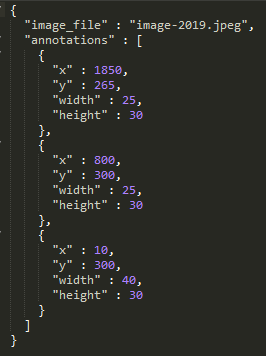
\includegraphics[width=.4\linewidth]{example_annotation}
    \caption{An example text file containing the annotation information used by Smok3 Tagg3r in the JSON format.}
    \label{fig:example_annotation}
  \end{figure}

Annotations are stored by Smok3 Tagg3r in .json files, although this is not a hard requirement of the program. Any text file containing valid JSON can be used by Smok3 Tagg3r.

%%%%%%%%%%%%%%%%%%%%%%%%%%%%%%%%%%%%%%%%%%%%%%%%%%%%%%%%%%%%%%%%%%%%%%%%%%%%%%%%
\section{Installation}
At this time, there is no `double-click installer' for Smok3 Tagg3r, but the installation and use of the program should still be relatively easy.

\subsection{Dependencies}
You will have to install the following dependencies for Smok3 Tagg3r to work.

\subsubsection{Python3}
First and foremost, you will need Python 3 installed on your machine. For best results, use Python 3.4.3. The Python 3 installer can be found at \texttt{https://www.python.org/downloads/}. Optionally, if you are using Mac or an Ubuntu-based Linux operating system, you might be able to use \texttt{sudo apt-get python3} in a terminal.

\subsubsection{Tkinter and PIL}
Tkinter is the library Smok3 Tagg3r uses for its GUI components. Tkinter itself should come packaged with your python distribution. However, for image support, you may need to install PIL, or better yet, a modernized version called Pillow.\\

If pip installed alongside your python installations (which it probably did), you should be able to open a command prompt on any operating system and use: \texttt{pip3 install pillow}. You may need to use \texttt{sudo} onMac or Linux, and if you run into trouble on windows, you can always try installing with the pre-compiled binary found at \texttt{http://www.lfd.uci.edu/~gohlke/pythonlibs/}.

\subsection{Installation and Usage}
Once the dependencies have been satisfied, you can `install' Smok3 Tagg3r. This should be simple for now. Simply download, unpack, etc. the code files as you have obtained them into an easy to reach directory.\\

If you do not have the program's files, you can find them on T-R0D's GitHub at: 
\begin{verbatim}
https://github.com/T-R0D/Smok3_Tagg3r
\end{verbatim}
There is a button on the right side of the page where you can download everything as a zipped folder is you are not accustomed to cloning GitHub projects.\\

Once the files are in placed where you want to keep them, open a terminal/command line prompt and navigate to that directory. Once your terminal is pointed at the `Smoke3Tagg3r' directory (with capital letters), run the program with the terminal command: \texttt{python smok3tagg3r.py} (with lower case letters).\\

  \begin{figure}[h!]
    \centering
    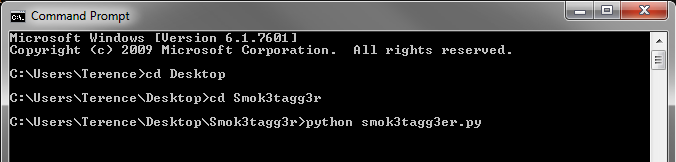
\includegraphics[width=.8\linewidth]{terminal_view}
    \caption{How a Windows command prompt would look as it is about to initiate Smok3Tagg3r.}
    \label{fig:menu_bar}
  \end{figure}

That's it! You should be up and running now and ready to annotate your images!\\

In the future I really do hope to get things packaged so that installation and usage is even more intuitive and natural. Updates will be posted to T-R0D's GitHub as soon as they are available.

%%%%%%%%%%%%%%%%%%%%%%%%%%%%%%%%%%%%%%%%%%%%%%%%%%%%%%%%%%%%%%%%%%%%%%%%%%%%%%%%
\section{How to Use Smok3 Tagg3r}
\subsection{The Menu Bar}
  \begin{figure}[h!]
    \centering
    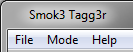
\includegraphics[width=.3\linewidth]{menu_bar}
    \caption{Smok3 Tagg3r's menu bar.}
    \label{fig:menu_bar}
  \end{figure}

The menu bar features $3$ menus:
\begin{itemize}
  \item \textbf{File}: Currently this menu is relatively useless - it only features an `Exit' option. In future versions of Smok3 Tagg3r this menu should gain functionality.

  \item \textbf{Mode}: This will likely be the most heavily used menu. This menu facilitates the switching between the `Tagging' and `Filtering' modes described below. There is not much to konw about this menu except that all data is discarded when switching modes, so be sure to save anything important before switching.

  \item \textbf{Help}: The help menu is a gateway to reading information about the application including information about the application and its author, the license the program operates under (don't worry - everything is free to use, distribute, modify, etc., we just want you to give credit where credit is due and not hold us liable for anything), and some brief instructions for using the application in case you don't have this document handy.
\end{itemize}

\subsection{Tagging Mode}
Tagging mode is for creating fresh, new labels or annotations for an image manually. Use this mode when you want a human to directly identify where areas of interest are in an image, such as where a face or smoke is.

  \begin{figure}[h!]
    \centering
    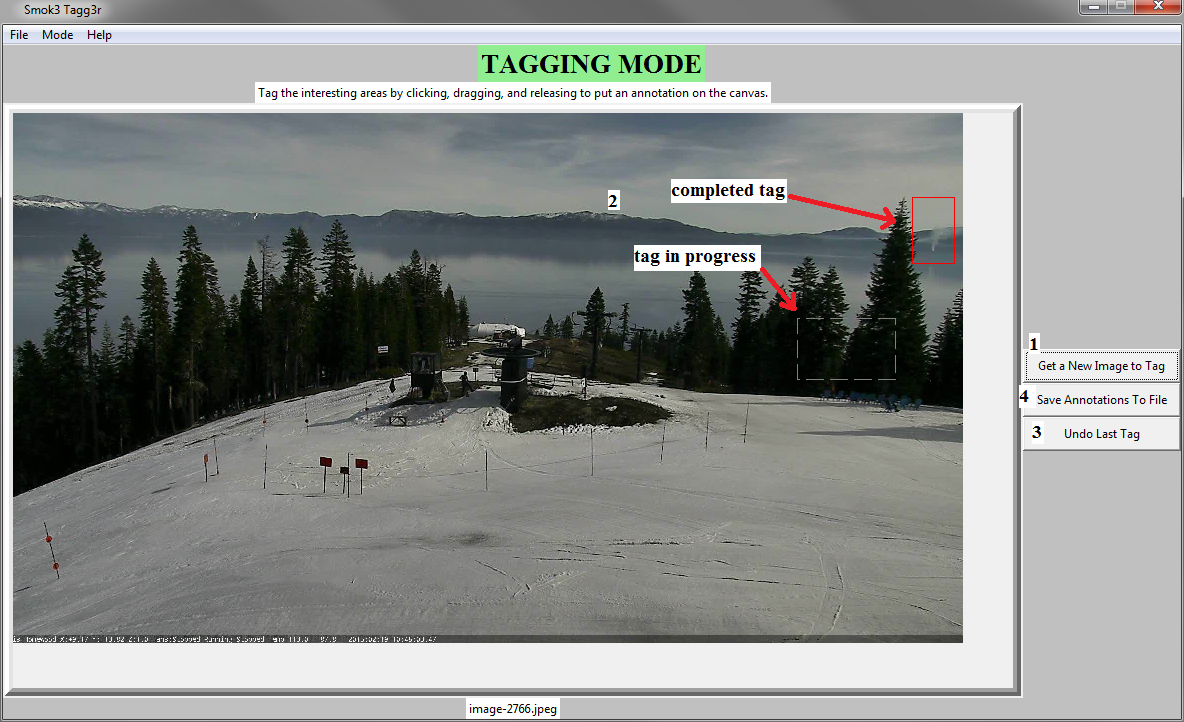
\includegraphics[width=.9\linewidth]{tagging_mode}
    \caption{Smok3 Tagg3r's tagging mode for original annotations.}
    \label{fig:tagging_mode}
  \end{figure}

\begin{enumerate}
  \item First you will need to get an image to tag. Click the `Get a New Image to Tag', select your image, and it is as easy as that. Do note that your image may appear as a scaled down version to fit in the window, but don't worry, the annotation data that is stored will be scaled back up when it is stored to match the original image.

  \item To create an annotation, simply click and drag to create a rectangle around the area of interest, and then release once the rectangle is properly drawn. While you are dragging and resizing your rectangle, a dashed rectangle should appear to guide you as you tag.

  \item But what if you messed up and drew a sloppy annotation? Don't worry, the `Undo Last Tag' button is there for you. Each time you click that button, the most recently added annotation will be removed and deleted. You can actually remove all annotations this way.

  \item Once you have drawn the sufficient annotations, you should save them to a file. On the right side there is a button labeled `Save Annotations To File'. Use it. You will be presented with a prompt asking you where to save the file. You can name the file anything, and preferably with the extension .json, but if you don't put .json, Smok3 Tagg3r will do so for you.
\end{enumerate}

\subsection{Filter Mode}
Filter mode is used to identify good and bad annotations. This mode was actually the first mode of the project developed because it might be the most practical. Filter mode was created with the intent that labeled data could be `bootstrapped'; that is, using preliminary methods, we can have a computer find areas of interest, and then reduce the human workload by having just a few areas for the human to consider rather than the whole image. It also allows us to identify images that are tricky for a classifier, so we can actually focus our trainging of classifiers to perform better on tricky inputs.

  \begin{figure}[h!]
    \centering
    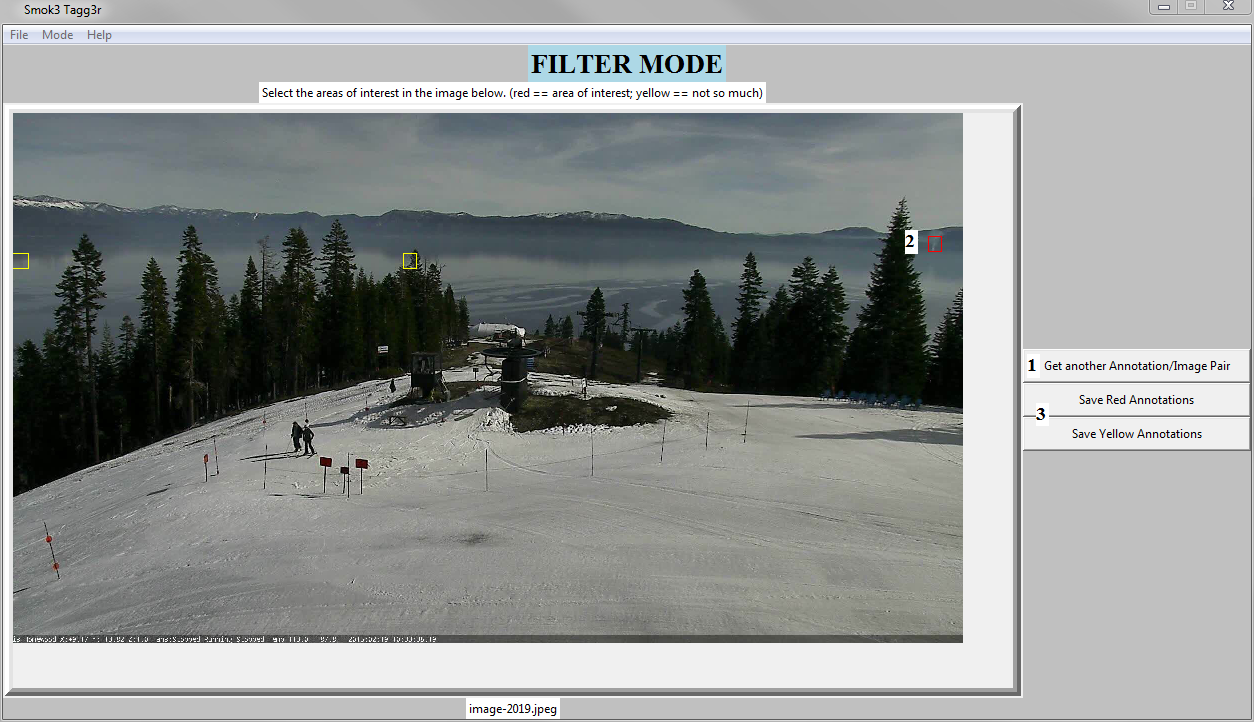
\includegraphics[width=.9\linewidth]{filter_mode}
    \caption{Smok3 Tagg3r's filtering mode for verifying annotations.}
    \label{fig:filter_mode}
  \end{figure}

\begin{enumerate}
  \item Start by clicking `Get Another Annotation/Image Pair'. This will present you with two dialog boxes, one after the other. The first dialog box wants you to locate an existing annotation file (likely a .json file). The second wants you to locate just the directory that the image file that corresponds to the annotation file is in. Smok3 Tagg3r can find the appropriate image file on its own at that point. Your use case might be different, but in the case that inspired the creation of Smok3 Tagg3r, this eliminates the need for a user to manually sift through thousands of image files that are contained in a folder. Again, the image appears, possibly scaled down. The annotations from the given file also appear n the image in yellow. Supplying files of the incorrect type will produce an error that the application will likely just ignore and you will have to try again.

  \item Now it's time to filter! Simply click the annotations that are `good' and they will turn red. If you change your mind, just click that annotation again and it will turn back to yellow.

  \item When finished, be sure to save your annotations. Use the appropriate button, `Save <color> Annotations', to save your annotations. Try to use appropriate names; it is recommended to save both sets. Again, you can add the .json extension to the names, or you can let it be added for you.
\end{enumerate}

%%%%%%%%%%%%%%%%%%%%%%%%%%%%%%%%%%%%%%%%%%%%%%%%%%%%%%%%%%%%%%%%%%%%%%%%%%%%%%%%
\section{Other Softwares of Interest for Similar Tasks}
Since Smok3 Tagg3r had to be developed so rapidly, it may not have as many awesome features as you might find you need. This is the tradeoff for Smo3 Tagg3r begin such a lightweight application. Also, it is uncertain how much maintenance or long term support Smok3 Tagger will get. Due to this fact, included here is a listing of some other softwares that might prove to be more feature rich, but will require a more involved setup (such as requiring a dedicated server or installing more dependencies than Smok3 Tagg3r requires.) I truly hope that Smok3 Tagg3r will be of use to you, but I would also hope that you are able to find the right tool for the job. These additional softwares are ranked in descending order of quality without regard for ease of use.\\

A quick digression is required. There is a service known as Amazon Mechanical Turk. This is a service for farming out tedious tasks that require humans to complete (referred to as Human Intelligence Tasks, or HITs). A task such as identifying areas of interest in an image when computers cannot (yet) is one such HIT. Mechanical Turk lets people from across the internet perform the HITs in exchange for a small monetary reward. Should you find yourself in need of a lot of cheap labor, this might be a place to look. Some of the softwares that are mentioned are already set up for integration with Mechanical Turk.

\begin{enumerate}
  \item \textbf{VATIC}: Video Annotation Tool from Irvine California can be found at \texttt{http://web.mit.edu/vondrick/vatic/}. This tool is a high quality tool designed for annotating multiple objects of multiple types in videos through time. It is also designed with Mechanical Turk in mind. Its use appears to be intuitive and smooth. However, it does require installation and deployment on an Apache server (meaning it is likely Linux-bound). This is a great software to consider if you plan to use video data and your project is going to be large in scale or long term. Otherwise you may consider it overkill.

  \item \textbf{LabelMe}: An image annotation tool for computer vision research from MIT (found at \texttt{http://labelme2.csail.mit.edu/Release3.0/index.php}). This tool has Amazon Mechanical Turk integration, seems to have significant Matlab support, and even offers an iOS app so labeling can be done from an iOS device if you choose. It appears that this application was designed for taking photos with an iOS device and uploading the images to a LabelMe cloud account, but it looks like images can be uploaded in the usual way (if you already had images of your own). LabelMe also looks like it is capable of building its own object detection for various classes of objects on an iOS device. This in and of itself is probably not very useful, but the software is open source, meaning that their code is available for free and the object detection code could be recycled to fit your own purposes.

  \item \textbf{Sloth}: Sloth can be found at \texttt{http://sloth.readthedocs.org/en/latest/index.html}. Sloth is lightweight and similar to Smok3 Tagg3r, but less wieldy and seems to be Linux-bound (I'm not certain of this). In fact, Sloth was a source of inspiration for Smok3 Tagg3r in that it invoked the feeling of ``This can be made easier." (That might be an issue of personal preference) Sloth's main advantage over Smok3 Tagg3r is its high level of annotation customization. Sloth allows users to define their own annotation classes that might be shapes other than rectangles or have special properties.
\end{enumerate}

%%%%%%%%%%%%%%%%%%%%%%%%%%%%%%%%%%%%%%%%%%%%%%%%%%%%%%%%%%%%%%%%%%%%%%%%%%%%%%%%
\section{Conclusion}
\subsection{The Future and Maintenance of This Project}
Unfortunately, it does not seem that Smok3 Tagg3r will see a lot of regular maintenance by its primary author. There is just not enough time in the week to make any promises of that sort. Plus, this project was meant to be quick and simple, so that the internals are not obfuscated from any users who need to integrate Smok3 Tagg3r into their project's pipeline.\\

That all being said, the project is stored on GitHub, which can really facilitate contributions from anyone who wants to offer up an improvement (for those unfamiliar with git/GitHub, this is referred to as a `pull request'). Literally anyone can offer a contribution to the project. Also, the original author, Terence, really wants Smok3 Tagg3r to fit might be willing to add features or perform fixes if they are `weekend tasks', meaning that the task might be possible to accomplish in 4 hours on a Sunday or something. A list of such tasks might include:
\begin{itemize}
  \item Add annotations of different color or the option to change the displayed colors of annotations.
  \item Fixing minor bugs that unexpectedly crash the application.
  \item Adding the capability for annotation shapes other than rectangles.
  \item Adding a zooming functionality for the image canvas (this might be more than a `weekend task')
  \item Adjustments to the storage of annotations.
  \item Adding support for an image format that doesn't seem to work as is.
\end{itemize}

\subsection{Concluding Remarks}
Smok3 Tagg3r was created in the hope that it would prove useful. I wish you the best in your use of this software, and should you ever need to contact me, Terence Henriod, with regards to this software I can be reached via my GitHub account \texttt{T-R0D} (that's a zero), or via email at \texttt{thenriod@gmail.com}.
%
\end{document}